\documentclass[12pt,a4paper]{article}
\usepackage{times}
\usepackage{durhampaper}
\usepackage{natbib}
\bibliographystyle{agsm}

\usepackage{graphicx}
\usepackage{float}
\usepackage{listings}
\usepackage[capitalize]{cleverref}
\crefname{lstlisting}{listing}{listings}
\Crefname{lstlisting}{Listing}{Listings}
\usepackage{syntax}
\usepackage{fancyhdr}
\usepackage{amsmath}
\DeclareMathOperator*{\argmin}{arg\,min}
\newtheorem{theorem}{Theorem}
\newtheorem{fact}{Fact}
\newtheorem{definition}{Definition}
\usepackage{wrapfig}

\setlength{\columnsep}{25pt}
\setlength{\intextsep}{0mm} 

\lstdefinelanguage{myLang}
{
  % list of keywords
  morekeywords={
    string, double, void, call, function,
    if, else, return, while, print, input
  },
  sensitive=true, % keywords are not case-sensitive
  morecomment=[l]{//}, % l is for line comment
  morecomment=[s]{/*}{*/}, % s is for start and end delimiter
  morestring=[b]" % defines that strings are enclosed in double quotes
}

\lstset
{
    language=myLang,
    basicstyle=\footnotesize,
    numbers=left,
    stepnumber=1,
    showstringspaces=false,
    tabsize=1,
    breaklines=true,
    breakatwhitespace=false,
}


\title{Automated bug detection}
\author{} % leave; your name goes into \student{}
\student{Abdul Ghani}
\supervisor{Stefan Dantchev}
\degree{BSc Computer Science}

\date{}

\begin{document}

\maketitle

\begin{abstract}
\par
\noindent
{\bf Context/Background.} The field of program verification, although fraught with undecidability, has still seen much success. Many techniques have been developed in order to
cope with different requirements and standards - for example, automated testing of 15K lines of video game code should differ from the formal verification of 600 lines
of safety-critical code.
\noindent
\par
\noindent
{\bf Aims.} The aim of this project is to implement graph-search algorithms in order to detect various bugs, i.e. misuse of arrays and loops that may not terminate. In particular we will focus on detecting `tired programmer errors' such as using unsanitized user input to index arrays and potential overflows.
\noindent
\par
\noindent
{\bf Method.} The user will write programs in a high level, procedural, C based language. This will be compiled into a Control Flow Graph (CFG) on which some standard
optimisations will be applied. Graph-theoretic algorithms will then be used in order to find feasible paths and detect loops. Along the way we will try to find executions
that lead to errors such as out of bound accesses, overflow and division by zero.
We will then try to determine the monotonicity of variables and certify termination (or 
infinite looping). The CFG will finally be translated into machine code for a state-based virtual machine.
\noindent
\par
\noindent
{\bf Results.} We had success in verifying termination of various looping programs, including recursive functions where termination is not immediately obvious (e.g. the Ackermann function). We were also able to certify nontermination of ruined versions of those looping programs as well as executions leading to the previously mentioned errors.
\noindent
\par
\noindent
{\bf Conclusions.} In this paper we describe a bug detection method that can be built into the compilation process. This method quickly discovers a range of errors.
\end{abstract}

\begin{keywords}
Program verification, symbolic execution.
\end{keywords}

\section{Introduction}
This paper describes the development of a compiler that attempts to verify certain desirable properties of the input during the course of the compiler.
This has been identified by Hoare as a `A grand challenge for computing research' \citep{hoare}.

Software has become the backbone of modern society.
The inevitable failures can be anything from annoying to costly to fatal - infamous examples are the failed Ariane 5 launch in 1996
(costing an estimated 7 billion dollars) and the patriot missile system (costing 28 lives).

Many diverse methods have been developed in order to detect them. The method of choice will depend on factors such as concurrency,
desired level of coverage, type 1 vs. type 2 errors, the size of the program, etc. The most thorough approaches invoke constraint solvers or satisfiability modulo theories engines. These approaches, although successful, are computationally expensive and may be overkill for non-safety-critical applications.

This project instead utilises techniques from the field of symbolic execution in order to overestimate the set of feasible paths through a program.
The idea is to try to maintain an upper and lower bound on the possible values of each variable, as well as basic relationships between variables.
These bounds are determined by conditions and arithmetic expressions (see~\cref{lst:ranges}).
We will then try to find paths through loops where progress towards breaking a loop condition can be guaranteed by tracking monotonicity of variables.

\begin{minipage}{\linewidth}
\begin{lstlisting}[caption=Example of ranges.,frame=tlrb, language=myLang, label={lst:ranges},escapeinside={(*}{*)}, numbers=none]
double x; (*\hfill $x = 0$ \hspace{100mm} *)
input x; (*\hfill $min \leq x \leq max $ \hspace{84mm} *)
double y = x % 8; (*\hspace{13.5mm} $ min \leq x \leq max,\quad 0 \leq y < 8$*)
if (y < 4)
{
  ... (* \hspace{38mm} $min \leq x \leq max,\quad 0 \leq y < 4 $*)
}
else if (x >= z)
{
  ... (* \hspace{38mm} $ min(z) \leq x \leq max,\quad 4 \leq y < 8, \quad x \geq z $*) 
}
\end{lstlisting}
\end{minipage}

In giving up constraint solvers we trade off accuracy for speed and flexibility.
We gain flexibility from the ability to symbolically simulate stacks and arrays, and we gain speed by determining path feasibility using depth first search.

The solution was implemented successfully. We managed to verify the termination of many small programs, some involving array usage and recursion.

\section{Related Work}
\subsection{Ranking functions}
A well founded partial order is a partial order where there are no infinitely decending chains. If we can find a \emph{ranking function} that maps successive loop iterations into a strictly decending chain we know that the loop must always halt.
This method was popularised by Floyd \citep{floyd}.

This method, although powerful and simple, is hard to automate. One attempt \citep{colon} begins by generalising the idea of a ranking function to strongly connected components (SCS) in a control flow graph - where now the ranking function is defined on the edges of an SCS, never increases on any edge, and strictly decreases on at least one edge. Every potentially loop must live in an SCS, as we can reach any node in the loop by following it around. We start by finding a ranking function (actually, a cone of such ranking functions, as if one exists there are infinitely many) for all the SCSs in a graph. We remove the edges where the ranking function decreases, as a nonterminating loop cannot use any of these edges. If the remainder of the component is not acyclic, we repeat the procedure.

This method is `sound' in the sense that if it succeeds in finding a ranking function for every SCS the program always halts. It may fail to find ranking functions
for programs that do infact halt.

\subsection{Term rewriting systems}
Briefly, a \emph{term rewriting system} which transforms an `object' into another `object' by applying transformation rules to `sub-objects'. This framework is very general and touches many ideas of fundamental importance in computer science (i.e., the lambda calculus, semi-Thue systems, grammars). The termination properties of such systems has therefore been very well studied \cite[p.~181]{zantema}.

Functional languages such as LISP and Haskell are amenable to interpretation as a rewrite system. Imperative languages, however, need more work. A method given in \citep{tra} takes the possible states of the program (the values of variables, including the program coutner) to be the objects and transforms each basic block into a rewrite rule, possibly enriched with a condition given in some logic. This method performs well on imperative programs without arrays and function calls, however
it does not provide immediate diagnostics on the cause of nontermination. The high level of abstraction also leads to something akin to the path divergence problem
discussed in the next subsection.

\subsection{Symbolic Execution}\label{revSymEx}
The last two methods are powerful but are not well suited to deal with arrays and function calls/stack usage. They also require `extra work' - transformations to, and manipulations of, structures and representations that are not in themselves useful to the compilation process. Many approaches search for bad execution paths by
simulating program execution, substituting symbolic representations of variables for concrete values. Each `probe' of the search will represent a range of possible program executions. As each
probe proceeds through the program it builds a path condition - the conjunction of conditionals it has taken. This method is named \emph{symbolic execution.}\\

\noindent
Anand \cite[pp.~2--3]{anand} identifies three issues with symbolic execution:\\
\begin{enumerate}
\item \textbf{Path explosion.} At every branch we may double the number of paths we must trace. While
nothing can be done about this combinatorial increase, We hope to lessen the damage by keeping the overhead
for each path as low as possible, by using simple constraints and appropriate data structures (see Section III.B below).\\ %todo check
Some other possible solutions are discussed. An interesting one is first summarising each basic block by how it affects certain variables.\\

\item \textbf{Complex constraints.} The path conditions generated may be intractable or even undecidable. Some more thorough program verifiers \citep{zhang, gupta}
invoke theorem provers and/or constraint solvers to try and determine the feasability of a path condition. This, while improving accuracy, will increase complexity
and running time.\\
In an attempt to deal with this, the intermediate language used to represent the control-flow graph will only
use conditionals with inequalities between a variable and another variable or constant value. More complicated expressions
will be compiled down into these simple conditions. We will then only maintain possible ranges for each variable. If a range of
a variable becomes empty, the path is not feasable.\\

\item \textbf{Path divergence.} Innacuracies will be inevitably introduced by modelling complex software with a simpler representation. Path divergence refers to the difference between the path followed by a symbolic execution of said model and the path that
should be followed in the code a programmer wrote. In our case, variables will have different names (as the state machine has no scope, variables will be renamed) and also it is
likely that compilation and optimisation will change the structure of the program to a significant degree. That being said, the representation
itself can be directly executed and so detected bugs will apply to the running program.
\end{enumerate}

\subsection{More similar work}
A similar approach to the solution presented here is the `lasoo' approach discussed in \citep{gupta}. It begins by symbolically executing the program and finding paths that revisit some state. It then uses a constraint solver to find states that are recurrent.

Another approach is the method discussed in \citep{loopster}. Like us, it tries to determine the monotonicity of variables in a loop execution. For each loop it builds a path-automata, where the nodes are paths and the edges possible transitions. Feasible cycles in this automaton are then executions of the loop that could run forever.
However, they don't use a symbolic engine, and cannot work with constructs such as call stacks and arrays.


\section{Solution}
\subsection{The approach}
\subsubsection{Compilation}
Most programs are developed using some high level language. We will be compiling and verifying programs written in a language based on PL/0, with the addition
of functions and function calls.

\begin{lstlisting}[frame=tlrb,language=myLang, caption=Fizzbuzz., label={fizzbuzz}, numbers=none]
while (current < limit)
{
 if (current % 15 == 0) print("FizzBuzz");
 else if (current % 3 == 0) print("Fizz");
 else if (current % 5 == 0)  print("Buzz");
 else print(current);
 print("\n");
 current = current + 1;
}
\end{lstlisting}

Programs in this form are easy for humans to read and write but harder for computers to optimise, test for bugs, and run. For this reason we will implement a small compiler that will translate the program into machine
code for a virtual machine.\\
Programs will be parsed in a top down predictive manner. The translation will be carried out during the parsing of the program. For this reason the parsing and translation will not be strictly context free - for example, the code generated
for a \texttt{return} statement will depend on the type of the function we are currently parsing.\\\par

 After translation the program will be held in memory as a Control Flow Graph (CFG):
 
\begin{figure}[H]
\centering
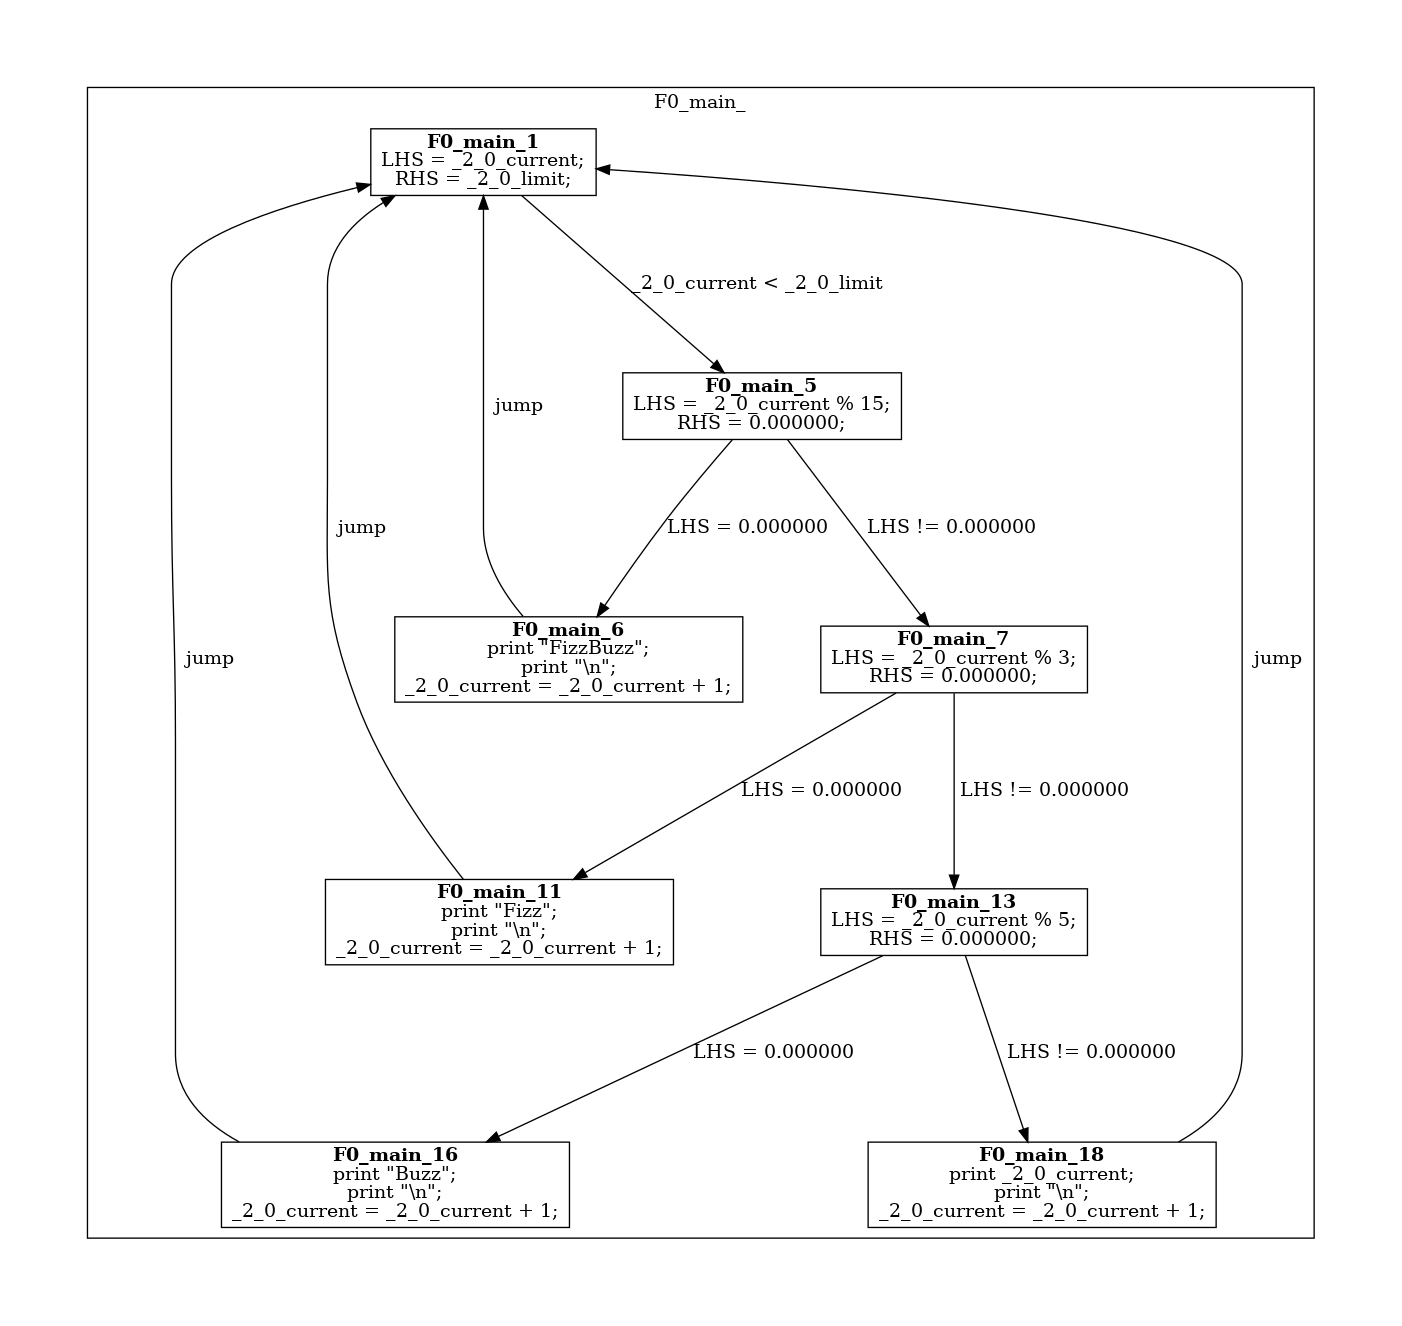
\includegraphics[width=0.7\textwidth]{images/fizzcfg}
\vspace{-1cm}
\caption{CFG for Fizzbuzz.}
\end{figure}

The nodes in the CFG are the so-called \textit{basic blocks} of the program - the sections of code that are always executed in sequence, containing no jumps.
These basic blocks can be seen as `states' in a pushdown-automata-like machine equipped with a stack (used for function calls), scopeless variables, and various (macros for) three address commands. Once we have the CFG, it's easy to translate into the description language of such a machine:

\begin{verbatim}
...
LHS = _2_0_current % 5;
jumpif LHS = 0.000000 F0_main_16;
jump F0_main_18;
end

F0_main_16
print "Buzz\n";
jump F0_main_1;
end
...
\end{verbatim}

The numbers in front of the translated variable names are to uniquely address variables in a scope free manner. See~\cref{app:spaghetti} for details of the implementation of the symbol table and the tagging of variables.

The CFG representation of a program is much more workable than the stream of characters initially received from the user. For example, it allows the compiler to perform certain optimisations.

\subsubsection{Dataflow and optimisation}
The flow of control, represented by the directed edges in the CFG, is a crucial element of most optimisation techniques. \textit{Data flow analysis} involves solving a system of equalities over some lattice, usually a power set ordered by inclusion. In the sections that follow,
$pred(n)$ denotes the incoming neighbours of a node $n$ in the CFG and $succ(n)$ its successors. $start$ will denote the entry of the CFG and $exit$ the exit.
\paragraph{Live variables}
 Say that a variable is \textit{live} at some point of the program if the value it is holding at that moment could be read later on (during any possible execution that passes through that point) and that it is \textit{dead} otherwise. We can remove statements using only dead variables,
as they can have no effect on the program. For each basic block $n$ we can simply iterate through its statements and calculate the sets of variables $used(n)$ (the variables used in that block) and $kill(n)$ (the variables
assigned and not read before the end of the block). The set of live and dead variables at each block then becomes
\begin{align*}
live(n)&= \left(\bigcup_{w\in succ(n)}live(w)\right) \setminus kill(n) \\
dead(n)&= used(n) \setminus live(n)
\end{align*}
and $live(exit) = \{\}$.

\paragraph{Assignment propagation}
It's useful to propogate assignments as far along as possible in a program. Doing so may let us simplify expressions and possibly remove conditionals.\\
Let $assignBasic(n)$ be the set of assignments leaving $n$ - for example, tuples of variable names and the values assigned to them. We can find variables safe to replace with the following equations:
\begin{align*}
assign(n)&= \left(\bigcap_{w\in pred(n)}assign(w)\right) \cup assignBasic(n) \\
assign(start)&= assignBasic(start)
\end{align*}
\paragraph{General formulation and solution}\label{par:general}
The two examples given are meant to demonstrate the similarities and differences found in data-flow problems. In the general framework introduced by Kildall~\citep{kildall} we find a least fixed point of some monotone function over a lattice.
Generally, each node monotonically transforms some input set $in(n)$ into an output set $out(n)$. They generate a set $gen(n)$ and kill a set $kill(n)$. The whole ordeal is then 
parameterized by the following variables:
\begin{enumerate}
  \item The actual `type' of the set elements - i.e., variables, expressions etc.
  \item \textit{Forward} vs \textit{backward} analysis. This refers to whether the set assigned to each nodes depends on its predecessors or its successors, respectively.
  \item \textit{Any} vs \textit{all} paths. This essentially dictates whether we work with unions or intersections when calculating $in(n)$.
  \item The initial output set $initOut(n)$ assigned to each node.
  \item The functions $gen(n)$ and $kill(n)$.
  \item The \textit{transfer function} $T_n$ at for each node $n$, which relates $in(n)$ and $out(n)$ \\(that is, $out(n) = T_n(in(n))$).
\end{enumerate}
This insight makes it possible to implement a general algorithm to solve a range of different dataflow problems.\par
A simple solution to this general formulation is the \textit{worklist algorithm}. We maintain a stack of nodes waiting to be processed. We pop nodes off this stack
and run their transfer function - if there is a change, we push the successors of that node onto the stack (`successors' here might be predecessors in the case of
backwards analysis).

\subsubsection{Symbolic execution}
Symbolic execution is an umbrella term encompassing many different techniques. The most careful maintain sets of symbolic equations of relationships between variables and employ solvers to see if the set is feasable. To reduce the running time of our program, and to ease implementation, we will instead maintain only simple relationships between variables (equalities and inequalities) as well as upper/lower bounds. Statements will then be allowed to manipulate this data. By a \textit{symbolic variable} we mean one of these indeterminate variables.

A symbolic execution of the program will be a search through the CFG. During the search we will maintain a \textit{state} which is just a set of symbolic variables and a symbolic stack. As we progress through a basic block we will affect the state as appropriate. 
When we reach a branch - which are the edges leaving a node - we may have to clone the state. This is because we cannot allow searches down independent paths to influence each other. Cloning the entire state on every branch would be wasteful and instead we adopt a `copy-on-write' approach discussed in~\cref{app:spaghetti.}

The verification procedure will consist of two searches. The first ignores how variables change and simply tracks the possible ranges of variables at each basic block of the CFG. A non-idempotent operation will affect the state as if it could be executed an arbitrary number of times. Similarly to data-flow analysis, we will carry on a search to the successors of some node $n$ only if we learn something new whilst searching $n$. Each node is tagged with the union of the ranges of variables in each visit. (For example, if a variable always happens to be nonnegative in a basic block this will be known.) Nodes that are never visited are then removed. After this stage, we carry out a more detailed
search through detected loops in order to produce certificates of termination/non-termination.

\paragraph{Improving variable-variable comparisons}
Say we encounter the condition \texttt{if} $(x < y)$. If we only restict the upper bound of $x$ so that it is less than the upper bound of $y$, we lose the potentially useful information that $x < y$.
We maintain this information by linking together symbolic variables with edges. We then retain those simple relationships between variables, and we also gain the ability to infer new relationships via transitivity.
As an example, if we hit the condition \texttt{if} $(x < y)$, but we have previously seen the conditions \texttt{if} $(x \geq z)$ and \texttt{if} $(z > y)$ we know we cannot enter.
If later we increase $x$ by a strictly positive amount, we forget all the less-than, less-than-or-equal-to, and equality edges leaving $x$ but keep the remaining.

\paragraph{Certifying termination of unnested while loops}\label{par:loops}
By a path through a loop we mean a simple path beginning with the loop header and ending with the exit. The path is essentially described by which conditions
in the loop body it passes and fails. For example, in \cref{fizzbuzz} there are $4$ paths, one for each \texttt{if/else} condition. We only inspect the first iteration, so there are only finitely many such paths.

We break each loop up into all possible paths from the entry to the exit. We will call a path \emph{good} if it makes progress towards leaving the loop,
possibly depending on user input, and \emph{bad} if it can repeatedly execute without making progress towards leaving the loop, independent of user input.
Essentially, we want to make sure no bad paths are ever executed, and we want to inform the user if we find this not to be the case.
This will involve producing a certificate showing the conditions taken at each branch.

\paragraph{Characterisation and extrapolation of the motion of variables}
As we search down one execution path of the loop we will try to find the most positive and most negative possible change of each variable. If both of these values
are positive (negative) we will guess that the variable increases (decreases) with every execution of the loop. After reaching the end of a path, we examine the 
variable involved in each loop condition encountered on that path and try to check that it moves towards that condition. (By `a loop condition' I mean any condition that leaves a 
node in the loop.) The path is called `good' if it moves towards any such loop condition.

It may be the case that for some number of loop iterations all relevant variables may be moving \textit{away} from the 
condition but eventually meet some \texttt{if} condition that kicks us out of the loop:
\begin{lstlisting}[frame=tlrb,language=myLang,label={lst:trickloop}, mathescape=true, numbers=none]
double n = 9;
while (n < 10)
{
  n = n - 1;
  if (n $\leq$ 0) n = 11;
}
\end{lstlisting}
This will be combatted by attempting to extrapolate the current motion of variables into the future. During a search we may encounter some condition
which the variable ranges forbid us from taking. So we first visit the second branch. If any execution of this branch always moves us towards meeting
this condition, we will go ahead and take it.

\paragraph{Nested loops}
It may be that one loop is nested inside another. We form an `inclusion tree', where the nodes are loops and an edge represents proper nesting. When we come to verify a loop in this tree we first recursively verify its children.
If we decide that they're bug-free we then verify the outer loop. When encountering the header of a nested loop, we update our symbolic variables with the overestimation formed during
the symbolic execution.\\

The method used to find the inclusion tree is adapted from a bioinformatical algorithm usually used to find perfect phylogenies \citep{gusfield}:

\begin{enumerate}
\item Assign each loop a bitvector, where the $i$th bit is $1$ iff the $i$th node appears in this loop.
\item Sort these bitvectors using radix sort.
\item For each loop, find the next highest loop that is is a superset and (if it exists) add this loop as a child. 
\end{enumerate}

\paragraph{Bug detection for arrays}
Arrays could be `symbolically simulated' by creating a symbolic variable for each cell - however this is obviously very wasteful. We instead maintain two lists - 
the first a list of indicies pointing to contiguous ranges which (as far as we can tell) have the same value, and the second a list of pointers to symbolic variables corresponding to those ranges.\\
For example, say the user creates an array of $10,000$ doubles. This array is represented
by a single symbolic double $init$ set to 0. Now the user adds $10$ to the cell with index $x$, $20 \leq x \leq 100$. We create a new symbolic double $nd$ with possible values $0 \leq nd \leq 10$.
The index list becomes $(20, 100)$ and the value list $(init, nd, init)$.

Given a undetermined index $i$ this symbolic array can then build a symbolic variable which represents our belief about the range of values present in the indicies spanned by $i$. It
can also emit a warning in the cases of potential out of bounds accesses.

\subsection{Symbol tables and spaghetti stacks} \label{app:spaghetti}
\subsubsection{The symbol table}
An easy way of handling scoped variables is to use a so-called \textit{spaghetti stack} \citep{dragon}. A spaghetti stack is usually a set of linked lists of hashtables (scopes), but during parsing we discard old scopes and only need a single linked list.\\
When a new scope is entered - which is marked by a \texttt{\{} - we create a new hash table and set it up to point to the previous one. New variable declarations are put in this table. If we declare a variable with the same name multiple times in the same scope, we will find that variable in the current scope and raise an error.\\
When we search for a variable, we first check the present scope. If it is not found there, we recursively search for it in the parent scope. If we end up running into a \texttt{nullptr}, we are trying to find a variable that has not been declared. Otherwise we will find and return the `most recent' declaration of that variable. Variables can be tagged with various data - some necessary for finding errors (i.e. type) and some useful for warnings (i.e. whether or not that variable has been defined).\\
When leaving a scope we delete the head of the spaghetti stack and forget every declaration that was inside. The symbol table keeps track of its current depth and the number of scopes it has processed in that depth in order to uniquely name each variable.

\subsubsection{Adapting the spaghetti stack for symbolic execution}
A small modification adapts the spaghetti stack into a structure useful for reducing memory used during symbolic execution.\\
During symbolic execution we will encounter conditions which may be true or false according to the information we currently hold. For example, we might be sure that $0 \leq i \leq 5$ and encounter the command \texttt{jumpif i >= 2 state.} We search the two different paths, one with $0 \leq i < 2$ and the other $2 \leq i \leq 5$. These two different branches must be independent in the sense that they cannot affect each other or future searches. One way of ensuring this would be to clone the entire state - duplicating every variable met so far. This is very wasteful, as the only difference at the moment is the single variable $i$.\par

A better way is to take advantage of the `most recent' property of searching through a spaghetti stack. Suppose we are using hash tables to map variable names to a \texttt{SymbolicVariable} object. Instead of duplicating that hash table for independent branches, we just set up two new hash tables with pointers to their parent. If we read a variable, we search up the spaghetti stack looking for the closest occurrence of that variable. If we change that variable in some way, we first copy it into the present table so that we don't affect other branches. This method has been used before (for example in KLEE - see \citep{klee}, Section 3.2).

\subsection{Finding loops in a CFG} \label{app:loops}
\subsubsection{What is a loop?}
\begin{figure}\label{fig:loops}
\begin{minipage}{.45\textwidth}
\begin{lstlisting}[caption=A loop.,frame=tlrb, language=myLang, label={isloop},numbers=none]
function main() void 
{call loopheader();}

function loopheader() void
{if (x < 10) call loopbod();}

function loopbod() void {
  print(x, "\n");
  x = x + 1;
  call loopheader();
}
\end{lstlisting}
\end{minipage}\hfill
\begin{minipage}{.45\textwidth}
\begin{lstlisting}[caption=Not a loop.,frame=tlrb, language=myLang, label={isnloop}, numbers=none]
while (1==1)
{
  return -1;
}
\end{lstlisting}
\end{minipage}
\end{figure}

We don't keep information about high level loop constructs when we move to the CFG representation, as not all `loops' are while loops and not all `while loops' are loops (see Listings \ref{isloop} and \ref{isnloop}). A tempting definition of a loop would just be a cycle, however this would be confused by branches within loops.\\
So how do we define a loop? We start by declaring that every valid execution that passes through a basic block in a loop must have passed through 
a `header' and will eventually pass out of some exit block.\par

\begin{definition}\label{def:dominator}
A node $a$ \emph{dominates} a node $b$ if every execution that passes through $b$ must have first passed through $a$.
\end{definition}

\begin{definition}\label{def:immediatedominator}
A node $a$ \emph{immediately dominates} a node $b$ if $a$ dominates $b$ and every node $n$ dominaiting $b$ also dominates $a$. Clearly it is unique, and we denote
the unique immediate dominator of $a$ as $idom(a)$.
\end{definition}

As the domination relation is antisymmetric and transitive it can be used to form the \emph{dominator tree} in which a node has as its children the nodes it
immediately dominates. The node then dominates everything in its rooted subtree.

\begin{definition}\label{def:backedge}
An edge in a CFG is a \emph{backedge} if its head dominates its tail.
\end{definition}

This is the normal definition of `back edge' in the dominator tree.

\begin{definition}\label{def:naturalloop}
The \emph{natural loop} of a backedge $n \to d$ is the set of all nodes that can reach $n$ without going through $d$. $d$ is the \emph{entry point} and $n$ the \emph{exit point.}
\end{definition}

Once we find dominators, we can easilly find natural loops by searching backwards from the exit point.

\subsubsection{Finding dominators}
We could compute the nodes that a node $n$ dominates by removing it and seeing which nodes become unreachable. We could also use an iterative approach, as the dominators of a node are  just the intersection of the dominators of its predecessors. However these algorithms are fairly slow and requires further work to find the immediate dominators.
The following algorithm, by Lengauer and Tarjan~\citep{lengtarj} is a better approach.\\
The algorithm begins by constructing a DFS tree of the CFG. As it does so, it labels the verticies in the order of arrival (i.e. preorder). Let $pre(n)$ denote the label given to node $n$, and $parent(n)$ its parent in the DFS tree.\\
After the nodes are labled, it computes `semidominators':

\begin{definition}\label{def:semidominator}
The \emph{semidominator} of $a$ is 
\[
\argmin\{pre(v) | v \to n_0 \to n_1 \to ... \to a, pre(n_i) > pre(a)\}
\]
That is, the semidominator is the least numbered node with a path to $a$
consisting of only higher labled nodes. Such a path is called a \emph{semidominator path.}
\end{definition}
We denote the semidominator of a node $n$ as $S_n$.
Semidominator paths can be used as counterexamples to one node dominating another. Intuitively, they `sneak around the right' of nodes in the DFS tree and prevent them from dominating nodes below. The semidominator can be thought of as the best possible counterexample.

We will need the following fact:
\begin{fact}\label{thm:semidominator}
If $semiNum(n)$ (the \emph{semidominator number} of $n$) is the label of the semidominator of $n$, then
\begin{align*}
semiNum(n) = \min(&\{pre(v) | V \text{ is a predecessor of $n$ with } pre(v) < pre(n)\}\\
\cup &\{semiNum(u) | u \text{ is a predecessor of $n$ with } pre(u) > pre(n)\})
\end{align*}
\end{fact}
Roughly, all of the immediate predecessors of $n$ are potential semidominators, with the higher labled ones being potential ends of semidominator paths. The semidominators of higher labled predecessors are also semidominators of the node itself. As the calculation of the semidominator depends only on the semidominators of higher labled nodes, we can start with the highest labled node and work downwards.\\
After calculating semidominators, we calculate the immediate dominators using the following fact:
\begin{fact}[\cite{lengtarj}, Corollary 1]\label{thm:imdominators}
Let $n \neq start$ and let $u$ be the node which minimises $pre(S_u)$ among all nodes $x$ satisfying $S_x \xrightarrow{+} x \xrightarrow{*} n$. Then:
\[
  idom(n) =
  \begin{cases}
  S_n & \text{if } S_n = S_u\\
  S_u & \text{otherwise}
  \end{cases}
\]
\end{fact}

\subsubsection{Implementation details}
As mentioned above we first process the nodes in decreasing DF order in order to calculate semidominators. We maintain for each node $n$ the set $bucket(n)$ of nodes
than $n$ semidominates.\\
The algorithm calculates semidominators using a union-find-like data structure. The trees in this structure will be fragments of the DFS tree formed earlier. It comes equipped with two functions:
\begin{align*}
link(v): &\text{ Connect $parent(v)$ with $v$ in the forest.}\\
eval(v): &\text{ If $v$ is the root of it's connected component, return $v$.}\\
   &\text{ Otherwise return a node $n$ with minimum semidominator number,}\\
   &\text{ such that $n \xrightarrow{*} v$,  not including the root.}
\end{align*}
Now $S_w$ is $\argmin\{semiNum(eval(n)) |n \to w\}$.\\
 After finding $S_w$ we place $w$ in $bucket(S_w)$. We then call $link(w)$ and link $w$ with its parent $parent(w)$ in the forest. Now we can implicitly find the immediate dominators of unprocessed nodes semidominated by $parent(w)$ (the nodes currently in its bucket) using~\cref{thm:imdominators.} 
 For each such node $v$ we calculate $u = eval(v)$. If $S_u = S_v$ then $idom(v) = parent(w)$. Otherwise, $idom(v) = idom(u)$. Note that in the second case we have only calculated $idom(v)$ \textit{implicitly} as we have not yet found $idom(u)$. 
 The bucket is then emptied.\\
Finally, after all the semidominators have been computed and the immediate dominators implicitly computed, we process the nodes in increacing DF order to fill in the blanks.\par

\subsection{Testing}
The purpose of writing a virtual machine for the produced machine code is twofold. The first is to combat the path divergence problem discussed in Section II.C. %todo check
It also allows us to observe the execution of the produced code and check that is runs as expected. The compiler was tested `by inspection' - the produced CFG and the
outputs of the compiled programs were checked manually for correctness.

Most of the testing of the verification software happened during collection of the results given in the next section. The examples were chosen so as to demonstrate all features of the solution,
and in doing so these tests achieve very high code coverage. In addition, the same examples were executed under the Valgrind debugging tool. This tool helps to detect memory leaks. More importantly, it can detect bugs that lead to undefined behaviour (these bugs might not have immediately obvious effects, but lead to problems later down the line).

Finally, unit tests were carried out on sufficiently moduar parts of the code - i.e., finding loops, radix sort, building symbolic variables that represent our beliefs about some array indicies,
etc.

\newpage
\section{Results}
The solution was exercised on various examples from the literature. Some of the examples have been reformatted (in superficial ways only)
 for brevity and readability.

\subsection{No functions}
Most of the following examples are taken from the appendix of \citep{tra}, itself a collection of examples from other papers.  All the examples given in this paper terminate, so we also introduced mistakes in order to test detection of nontermination.

\subsubsection{Bubblesort}
\begin{wrapfigure}{r}{0.4\textwidth}
\centering
\begin{lstlisting}[frame=tlrb,language=myLang]
while (x > 0){
 double y = 0;
 while (y < x){
  if (a[y] > a[y+1])
    swap (a[y], a[y+1])
  y = y + 1;
 }
 x = x - 1;
}
\end{lstlisting}
\end{wrapfigure}
This bubblesort implementation was correctly determined as halting. The programs obtained by removing any of the update lines, or moving either of the variables the wrong way, or inverting any of the equalities on lines $1$ and $3$, were correctly detected as nonterminating with an explanation given. Changing the comparitor in line $3$ from $<$ to $\leq$ results in an out of bounds access, which was successfully picked up.\\

\subsubsection{Two variables \cite[A.6]{tra}}

\begin{wrapfigure}{r}{0.3\textwidth}
\centering
\begin{lstlisting}[frame=tlrb,language=myLang]
while (x > y + z){
 y = y + 1;
 z = z + 1;
}
\end{lstlisting}
\end{wrapfigure}
This example was correctly detected as terminating. It also picked up the potential overflow in all three additions.
The comparison in line $3$ is compiled into the three-address-code \texttt{RHS = y + z, jumpif x > RHS ...}
We then need to use `transitivity properties' to classify this sample as halting - the inequalities \texttt{x > RHS = y + z},
and the fact that if \texttt{y} and \texttt{z} are increasing then so is \texttt{RHS.}
Changing any of the increments in lines $2-3$ to decrements, and inverting the inequality in line $1$, are detected as infinite loops with good reasons given.

\subsubsection{Relative change \cite[A.8]{tra}}

\begin{wrapfigure}{r}{0.3\textwidth}
\centering
\begin{lstlisting}[frame=tlrb,language=myLang]
while (x > y){
 x = x + 1;
 y = y + 2;
}
\end{lstlisting}
\end{wrapfigure}
Both variables in this example are increasing - the loop only halts as \texttt{y} is increasing faster than \texttt{x.}
This is noted by the program and it is classified as termiating. Inverting the condition, or swapping the constants in the addition,
results in a nonterminating program that is detected.

\pagebreak
\subsubsection{Multiplication \cite[C.1]{tra}} \label{mult}

\begin{wrapfigure}{r}{0.35\textwidth}
\centering
\begin{lstlisting}[frame=tlrb,language=myLang]
while (x >= 0) {
 double y = 1;
 while (x > y) y = 2 * y;
 x = x - 1;
}
\end{lstlisting}
\end{wrapfigure}
In this example, the inner loop is seen to terminate (as y is increasing) and then the outer loop follows (as x is decreasing).
Replacing the $2$ in line $4$ with a positive constant less than $1$, or inverting any of the comparisons, results in a detected nonterminating program.

\subsection{Calls and recursion}
\subsubsection{The Ackermann function}\label{example:ack}
\begin{wrapfigure}{r}{0.4\textwidth}
\centering
\begin{lstlisting}[frame=tlrb,language=myLang]
function ack(double m, double n) double
{
 if (m <= 0) return n + 1;
 else if (n <= 0) 
  return ack(m-1, 1);
 else {
  double a = ack(m, n-1);
  return ack(m-1, a);
 }
}
\end{lstlisting}
\end{wrapfigure}
This function halts, as it is always called on strictly decreasing pairs (in the lexicographic ordering).
Changing the decrement in lines $5$ and $7$ into an an addition of a nonnegative constant is correctly seen to be nonterminating,
however the method fails to detect the same when line $8$ is modified.

This function is normally defined on the natural number, and the inequalities are given as equalities - doing so here results in a potentially
nonterminating input, as $m$ and $n$ might both be negative.

\subsubsection{McCarthy's 91 function}
\begin{wrapfigure}{r}{0.4\textwidth}
\centering
\begin{lstlisting}[frame=tlrb,language=myLang]
function m(double n) double
{
    if (n > 100) return n-10;
    else{
        n = n + 11;
        return m(m(n));
    }
}
\end{lstlisting}
\end{wrapfigure}
This function is a standard exercise for automated termination analysis methods. Changing the expression in line $5$ into subtraction of a negative constant,
or inverting the condition in line $3$, result in nonterminating programs that are successfully detected by the method.

\begin{minipage}
\subsubsection{Greatest common divisor}
\begin{wrapfigure}{r}{0.4\textwidth}
\centering
\begin{lstlisting}[frame=tlrb,language=myLang]
...
	if (m <= 0 || n <= 0) return -1;
	double result = gcd(m, n);
...

function gcd(double m, double n) double
{
	if (m == n) return m;
	else if (m > n) return gcd(m - n, n);
	else return gcd(m, n - m);
}
\end{lstlisting}
\end{wrapfigure}
This is correctly determined as halting, as each parameter moves in a direction that takes us out of that control path (i.e., if $m > n$ and $m$ is decreasing eventually $m \leq n$).

Reversing the inequality on line $9$, or the order of the parameters in either of the recursive calls, is picked up as nonterminating - but not if we remove the nonnegativity condition
imposed on line $2$.
\end{minipage}
\pagebreak
\section{Evaluation}
\subsection{Evaulation of the method}
\subsubsection{Pluses}
As shown in the previous section the solution successfully verified a diverse range of programs, and did not struggle with array usage and/or function calls.
We also managed to detect a variety of bugs - overflows, out of bounds accesses, and potential infinite loops. The method is especially good at detecting simple (yet common) errors - such as off by one errors, wrongly assuming that variables are in a certain range
(i.e. that a user input is nonnegative), equalities that are the wrong way around, and forgotten/misplaced loop counter increments.

It is also worth noting that this method is mostly independent of the source language itself, as long as it is imperative. It requires only a control flow graph of the produced target machine code (which is
constructed in every compilation process that the author knows of) and the effects of each machine code statement on the state of the machine, which only need to be programmed once.

The fact that the method only needs a data structure produced anyways during compilation means that it is easily built into the compilation process. Symbolic execution
itself can me used to further optimise code, for example by detecting infeasible code or useless operations.

Finally this method is very easy to use, as the only input it requires from the user is the source program, and it runs automatically in the background. It does
not require any modifications to the source code (i.e. annotations given in first order logic), and it does not have any learning curve (i.e. it is not a separate
program with many commands and operating modes \`a la Valgrind/GDB). 

\subsubsection{Minuses}
\textbf{Path dependencies.} As long as we think we can leave a path we call it terminating. Consider now two paths that can alternate forever, or
one path that once entered can be left but will be revisited infinitely often - our method falsely accepts these cases as terminating.

An approach discussed earlier \citep{loopster} builds a graph where the nodes are loop paths and the edges possible transitions between the paths, annotated with
conditions that must be met for this transition to take place. Our method ony looks for nodes with only self loops - a better approach would look for feasible cycles.

\textbf{Short sightedness.} Our method extrapolates as much as possible by inspecting the behaviour of the variables only on the first iteration. Complicated loops can exhibit behaviour that requires more work to uncover. For example, a variable may be decremented by another variable that is begins positive but is itself
decreasing:

\begin{center}
\begin{minipage}{5.5cm}
\begin{lstlisting}[language=myLang, frame=tlrb, numbers=none, label={lst:termin}, linewidth=5cm]
double d = 5;
while (x < y){
	x = x - d;
	d = d - 1
}
\end{lstlisting}
\end{minipage}
\end{center}

The solution would declare $x$ decreasing and the loop nonterminating, although this is not the case.\\

\textbf{Inequalities.} Our method declares an inequality condition eventually broken if there is any relative change between the left and right hand sides.
It's correct to say that if all there is no relative change between both sides of an equality it will hold forever, however this is not necessary for a nonterminating loop.
For example, the method accepts as halting the probematic code fragment
\begin{center}
\begin{minipage}{6.5cm}
\begin{lstlisting}[language=myLang, frame=tlrb, numbers=none, linewidth=6cm]
double x = 1; double y = 0;
while (x != y) x = x - 2;
\end{lstlisting}
\end{minipage}
\end{center}

\textbf{Type 1 and 2 errors.} In this paper we have given an example of a nonterminating fragment that the program accepts as terminating (our modification to the
Ackermann function) and a terminating fragment we deem nonterminating (\cref{lst:termin}). This unfortunately means that you cannot believe either decision and must
inspect any diagnostic output manually.\\

\textbf{Division and multiplication.} Our method works well with linear increments. It does not perform as well with multiplication and division, as it only extrapolates
from the change that occurs first iteration. For example, in the multiplication example given above (\cref{mult}) it sees that $y$ increases from $1$ to $2$
and assumes wrongly this will continue forever. More generally, if a variable must be in the range $[l, u]$ and it is multiplied by a nonnegative constant $c$ it is now in the range $[cl, cu]$. If $l$ is nonnegative the method will correctly deduce that that variable is increasing but incorrectly proceed as if that variable is increasing by the same increment each loop. This is an area where a true, high resolution symbolic representation would be useful.

\subsection{Issues during the implementation and development process. Lessons learned.}

\textbf{Adding unused generality.} The biggest and most painful lesson I learned during the project was the harm caused by the addition of extraneous and unnecessary features (known in the SE community
by various related dicta such as Feature Creep, Keep It Simple Stupid, and You Ain't Gonna Need It).

Initially I planned to only allow programs with the single variable type
of double precision floating point. However, after writing the symbolic execution engine, I noticed that it would not take much work to extend the symbolic execution phase to work with any
data type that can be ordered. This was indeed true and the implementation of the extention was made easy by the use of templates.

The issues began when I came to implement the loop validation phase. In this phase we try to determine the motion of variables - however not every ordered type can be `incremented' in the way doubles can (i.e. strings). This lead to the use of type flags, downcasting to subclasses according those type flags, and methods in the
base class which have empty implementations in derived classes. This probably could have been prevented via more thoughtful OOP design, but the best solution would
have been to not implement them in the first place.

Towards the very end of the development of the project I decided to remove the functionality entirely. The relevant git commit registers
$1349$ insertions and $2199$ deletions - such an invasive operation has left its scars on the quality of the code.
\\

\textbf{Implementing a compiler.} For this project I decided to write my own compiler. This was a valuable learning experience. It also did not take much time and effort, as the compiler is small
and uncomplicated. However, using an existing compilation toolkit (such as LLVM) would have taken a similar level of effort and would have provided several benefits,
stemming from the ability to parse `real' languages.

The simplicity of the compiler means that the source language is necessarily constrained, For example, my compiler doesn't support 
expressions in function parameters or array indicies. Verifying programs written in real, practical languages would have made collecting results easier, and more 
importantly could have found immediate real-world use (especially if it was built into a popular toolchain).

Also, for comparison purposes it would have been interesting to see how this method
compares to other methods. The benchmark of choice is SV-COMP \citep{svcomp}, which publishes their test set as well as previous results and running times. These
test sets are written in C, which I could have tried the method on if I used a toolchain.\\

My supervisor was sceptical about both of these things - there is a third lesson to be learned here, too.

\section{Conclusions}
This paper has described a method that catches a wide range of program errors. For diagnostic and correction purposes it produces annotated execution traces that lead
to the error occuring. It can deal with array usages and function calls. Finally, it works only with structures produced during the compilation process
and can itself be seamlessly built into a compiler, without any extra work required from the user. 

\subsection{Future work}
\textbf{Addressing the issues discussed in the previous section.} None of the issues mentioned there are fundamental to the method.\\

\textbf{Extention to other programming paradigms.} The solution as described works with imperative languages only - we affect some global state as we proceed through
the program and through loops. The principles underlying the technique given here could be extended to stateless paradigms, such as functional and logic programming.\\

\textbf{Assertions.} Assert statements are statements inserted into code that give an invariant condition that is expected to hold at that line - i.e., $x \geq 0$.
During the execution of the program these statements are checked for their validity - if an assertion is found to not hold the program is halted. It would not be hard
to use this method, or symbolic execution in general, to automatically search for program executions where an assertion does not hold.\\

\textbf{Constraint solvers.} We avoided the use of constraint solvers for speed and flexibility. There are, however, many cases where speed can be sold in
exchange for accuracy and thoroughness. In these cases it may be profitable to combine the method given here with constraint solvers - doing so would retain the flexibility
afforded by symbolic execution (i.e. the simulation of stacks and memory) but give us much more power to detect feasible/infeasible paths and monotonically changing variables. The assertions just discussed could be enriched with the constraint language chosen, and we would be able to check additional, custom properties (such as
`Bubblesort actually sorts').\\

\textbf{Memory.} The method could be easily extended to search for null pointer dereferences and memory leaks. Some more work, possibly using similar techniques to the ones used to simulate arrays, could be used to simulate the contents of memory and allow for pointers to be used just like other variables.\\

\textbf{Decomposition, summarisation, and re-compilation.} At present we run the method on the entire CFG of the input program. This would take a very long time for
large, real world programs. If we change a single line in the program we are forced to re-verify its entirety.
 
 A better approach might split up the program into constituent functions, loops, or otherwise dense subgraphs of the CFG. It might then verify each independently, finding some way to approximate
 the sparse interactions between the segments. An approach like this is `loop summarisation' as discussed in \citep{summary}, where nested loops are replaced by summaries that over-approximate their effect on the state. 
\bibliography{projectpaper}

\end{document}
